\section{Experimental Results}
\label{sec:experimentalResults}

\subsection{Curriculum learning with aerial imagery}
\label{sec:results_curriculum_learning_aerial_imagery}

\begin{figure}[!ht]
\begin{subfigure}{0.48\textwidth}
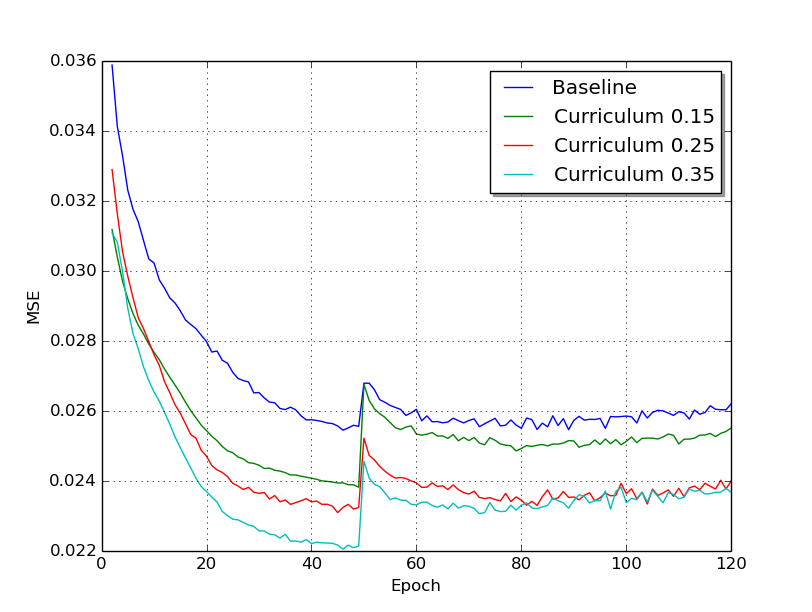
\includegraphics[width=\linewidth]{figs/E1/E1-lc.png}
\caption{Comparison of test loss} \label{fig:E1_curr_norway_loss}
\end{subfigure}
\hspace*{\fill} % separation between the subfigures
\begin{subfigure}{0.48\textwidth}
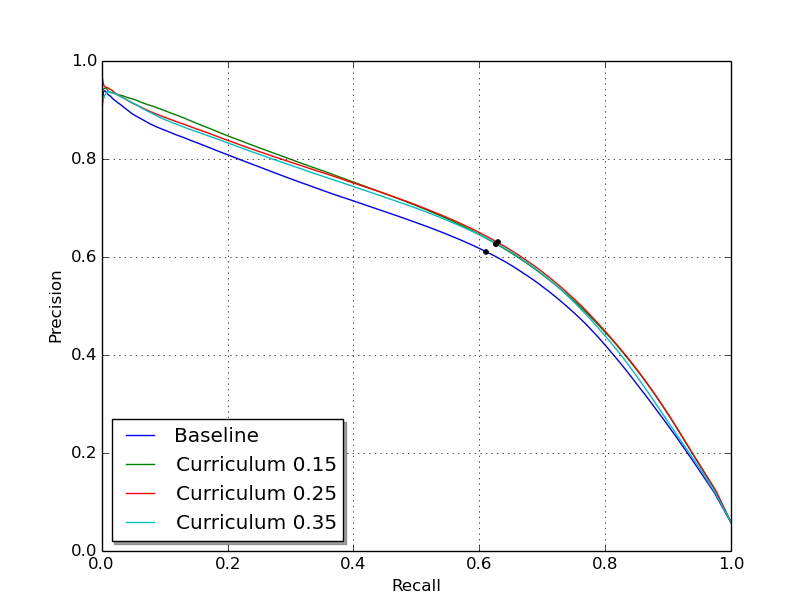
\includegraphics[width=\linewidth]{figs/E1/E1-pr.png}
\caption{Precision and recall comparisons.} \label{fig:E1_curr_norway_pr}
\end{subfigure}
\hspace*{\fill} % separation between the subfigures
\caption{E1 - Performance of curriculum learning at different thresholds, $D_{0}$ for Norwegian Roads Dataset Vbase} \label{fig:E1_curriculum_norway}
\end{figure}

In Experiment E1, the road detection system have been trained on four different patch datasets. The system's performance for each of these datasets are displayed in Figure \ref{fig:E1_curriculum_norway}. A comparison of the test loss per epoch is displayed in Figure \ref{fig:E1_curr_norway_loss}, whereas the final performance of each network is shown by a precision and recall curve in Figure \ref{fig:E1_curr_norway_pr}. The network configuration used for the tests was identical, as well as the number of training examples seen while training. The performance gap between the results, comes from the first stage of the patch datasets, where different difficulty threshold $D_0$ have been used.\\



Observing the plots in Figure \ref{fig:E1_curr_norway_loss}, the switch between stage 0 and stage 1, is clearly visible at epoch 50. The increase in test loss is most severe in the datasets formed by a curriculum strategy. Leading up epoch 50, the curriculum plots show an increasing gap in test performance against the baseline plot. After the switch the curriculum datasets still outperform the baseline dataset, even though the training set distribution of stage 1 are the same for all patch datasets.\\

Furthermore, the networks trained with a curriculum strategy shows an improved precision for all levels of recall compared to the baseline. \todo{Not so different here}\\

An interesting trend between the thresholds $D_0$ and the loss, is that decreasing the difficulty threshold, does not necessarily produce better results. The patch dataset \textit{Curriculum 0.15} has the easiest first stage, yet performs worse than \textit{Curriculum 0.25} and \textit{Curriculum 0.35} \todo{Generalize, easier examples reduce variability of training set, generalize worse. Discussion?}. \\

\todo[inline]{Need to place distribution charts somewhere}


A similar experiment was also performed on the Massachusetts Roads Dataset. In Experiment E2, networks are trained with three different patch datasets. The first stage of the baseline dataset have a first stage constructed by random sampling, which means that no examples were filtered out because of estimated difficulty. The curriculum dataset has a difficulty threshold $D_0$ of 0.25, which exclude every example with a estimated difficulty above 0.25 from the first stage. In contrast, the anti-curriculum patch dataset only have examples with a difficulty above 0.25 \todo{Mention, the non-road patches, and why non-road examples have been included}.\\


The results from this experiment can be seen in Figure \ref{fig:E2_curriculum_mass}. The switch from stage 0 and stage 1 is visible for the \textit{Baseline} and \textit{Anti-curriculum} loss plots at epoch 50. The network trained with the dataset constructed with a curriculum strategy, performs better than the baseline as seen in Figure \ref{fig:E2_curr_mass_loss} and Figure \ref{fig:E2_curr_mass_pr}. Training with an anti-curriculum strategy, where the first stage consists of harder examples, does not provide the same loss, or breakeven. This is especially evident in the plot of test loss, where the network converge around epoch 25, and start to overfit slightly towards epoch 50. From epoch 50 when stage 1 examples entered the training set, there is a dramatic decrease in test loss. The final performance of anti-curriculum learning is substantially lower than both baseline and curriculum learning, as illustrated by the breakeven points in Figure \ref{fig:E2_curr_mass_pr}.\\

The precision and recall breakeven values from Experiment E1 and Experiment E2, are listed in Table \ref{tab:results_curriculum_learning_breakeven}, and shows that training with a curriculum dataset is beneficial for both datasets.\\
\begin{figure}[!ht]
\begin{subfigure}{0.48\textwidth}
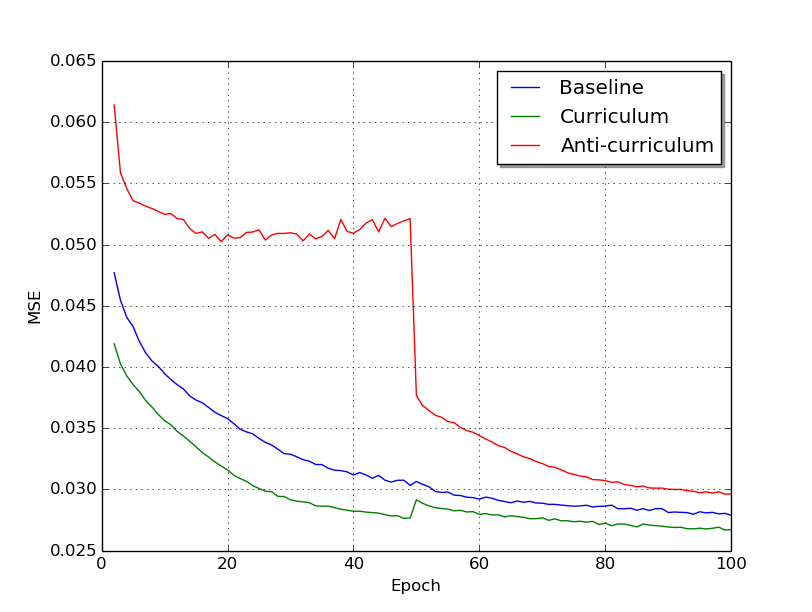
\includegraphics[width=\linewidth]{figs/E2/E2-lc.png}
\caption{Comparison of test loss} \label{fig:E2_curr_mass_loss}
\end{subfigure}
\hspace*{\fill} % separation between the subfigures
\begin{subfigure}{0.48\textwidth}
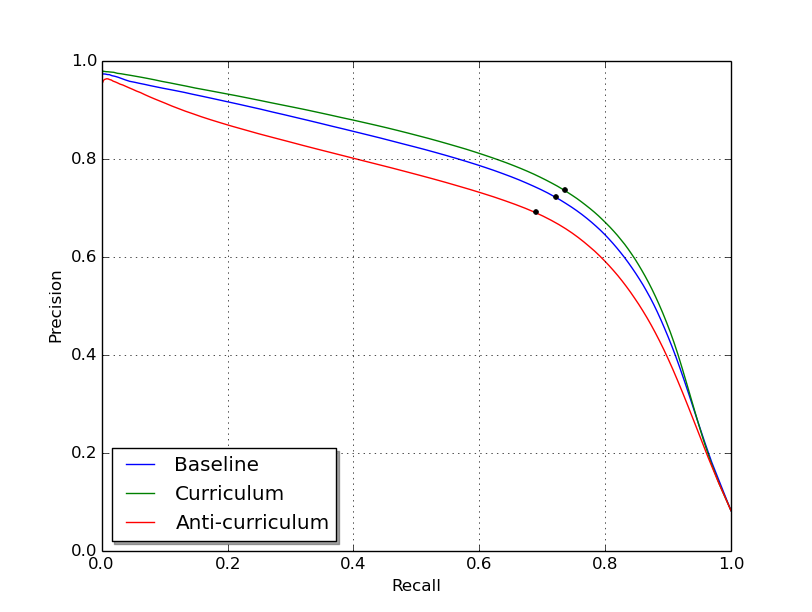
\includegraphics[width=\linewidth]{figs/E2/E2-pr.png}
\caption{Precision and recall comparisons.} \label{fig:E2_curr_mass_pr}
\end{subfigure}
\hspace*{\fill} % separation between the subfigures
\caption{E2 - Performance of curriculum learning and anti-curriculum learning for Massachusetts Roads Dataset} \label{fig:E2_curriculum_mass}
\end{figure}

\begin{table}[!ht]
\caption{Curriculum learning results.}
\begin{center}
\begin{adjustbox}{max width=\textwidth}
\begin{tabular}{+l ^l ^l ^r}\hline
\rowstyle{\bfseries}
  Experiment & $\mathbf{D_0}$ & Dataset & Breakeven\\\hline
  Baseline & 1.0 & Norwegian & 0.6105 \\
  Curriculum &0.15 & Norwegian & 0.6264 \\
  Curriculum &0.25 & Norwegian & \textbf{0.6292} \\
  Curriculum &0.35 & Norwegian & 0.6269 \\\hline
  Baseline &1.0& Massachusetts & 0.7211 \\
  Curriculum &0.25& Massachusetts & 0.\textbf{7353} \\
  Anti-curriculum &0.25 & Massachusetts & 0.6904 \\\hline
\end{tabular}
\end{adjustbox}
\end{center}
\label{tab:results_curriculum_learning_breakeven}
\end{table}

\subsection{Bootstrapping for imagery with noisy labels}
\label{sec:results_bootstrapping}

The results from comparing the bootstrapping methods and the baseline method at several levels of label noise, are displayed in Figure \ref{fig:E3_boot_mass} and Figure \ref{fig:E5_boot_norway}. The plots in the first figure are based on models trained on the Massachusetts Roads Dataset, whereas the second figure show results from training on the Norwegian Roads Dataset. The label noise have been artificially added to the label images before training. Specifically, areas of road pixels have been removed incrementally, by setting the label pixel values to zero. This process is continued until a certain percentage of road class pixels have been removed. In terms of aerial imagery, the artificially added label noise simulate omission errors, in which roads have not been marked in the label maps. Experiment E3 and E5, utilized patch datasets where 0, 10, 20 ,30 and 40 percent were removed from the labels.\\

\begin{figure}[p]
\begin{subfigure}{0.48\textwidth}
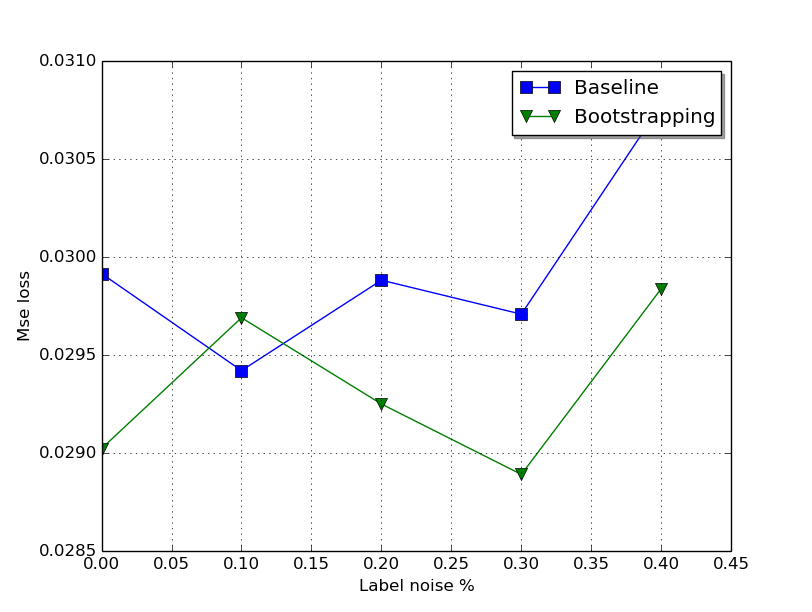
\includegraphics[width=\linewidth]{figs/E3/E3_lc_noise.png}
\caption{MSE test loss} \label{fig:E3_boot_mass_loss}
\end{subfigure}
\hspace*{\fill} % separation between the subfigures
\begin{subfigure}{0.48\textwidth}
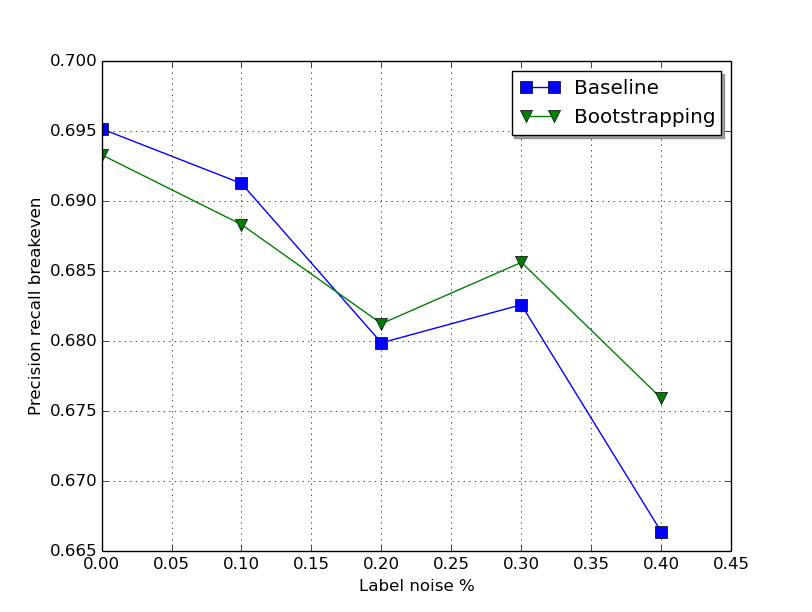
\includegraphics[width=\linewidth]{figs/E3/E3_pr_noise.png}
\caption{Precision and recall breakeven} \label{fig:E3_boot_mass_pr}
\end{subfigure}
\hspace*{\fill} % separation between the subfigures
\caption{E4 - Robustness of bootstrapping for increasing amount of label noise. Massachusetts Roads Dataset} \label{fig:E3_boot_mass}
\end{figure}

\begin{figure}[p]
\begin{subfigure}{0.48\textwidth}
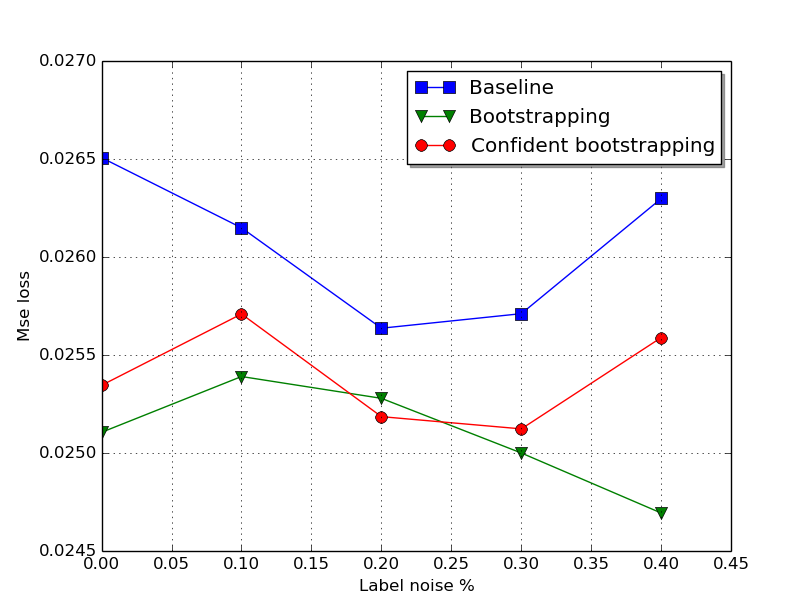
\includegraphics[width=\linewidth]{figs/E5/E5_lc_noise.png}
\caption{MSE test loss} \label{fig:E5_boot_norway_loss}
\end{subfigure}
\hspace*{\fill} % separation between the subfigures
\begin{subfigure}{0.48\textwidth}
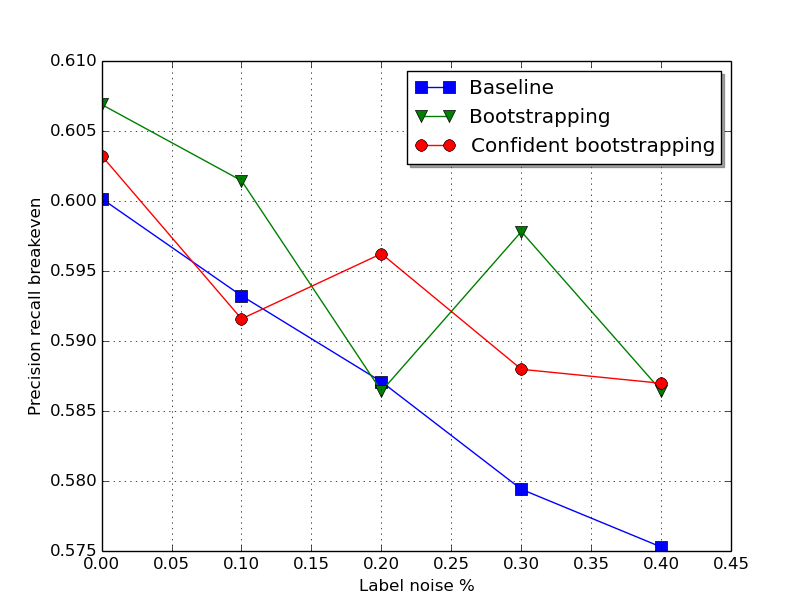
\includegraphics[width=\linewidth]{figs/E5/E5_pr_noise.png}
\caption{Precision and recall breakeven} \label{fig:E5_boot_norway_pr}
\end{subfigure}
\hspace*{\fill} % separation between the subfigures
\caption{E3 - Robustness of bootstrapping for increasing amount of label noise. Norwegian Roads Dataset} \label{fig:E5_boot_norway}
\end{figure}

In Experiment E3, conducted on the Massachusetts Roads Dataset, Figure \ref{fig:E3_boot_mass_loss} displays the averaged test loss at different levels of label noise. Generally, the baseline, which utilize the cross-entropy, seems to increase in test loss, as the noise level is increased. The bootstrapping loss function has a lower test loss for noise levels above 10 percent.\\

Figure \ref{fig:E3_boot_mass_pr}, which displays the precision and recall breakeven values at increasing levels of label noise, shows a trend of decreasing values. For label noise levels above 20 percent, bootstrapping surpass the baseline. Though, the difference in performance is limited.\\

The same type label noise experiment has been conducted for the Norwegian Roads Dataset as well, and include a plot of the confident bootstrapping performance. In Figure \ref{fig:E5_boot_norway_loss}, the test loss for bootstrapping and confident bootstrapping are consistently lower than the baseline. As expected, the precision and recall breakeven points for the baseline, decrease with increasing levels of omission noise. This can be seen in Figure \ref{fig:E4_boot_norway_vbase_pr}. Although the bootstrapping methods behave a bit more erratic, they generally tend to decrease at a slower rate \todo{A bit hard to see, doncha think!}.\\

A slightly different approach has been taken for Experiment E4. The road detection system has in this experiment been trained with a labels from the label set N50. This label set have a higher rate of omission and registration noise, than the labels in Massachusetts Roads Dataset for instance. The test set however, consists of labels originating from the Vbase label set, which is more accurate. The result from this experiment is displayed in \ref{fig:E4_boot_norway_vbase}\\

\todo[inline]{Explain what the figure shows.}

  
\begin{figure}[!ht]
\begin{subfigure}{0.48\textwidth}
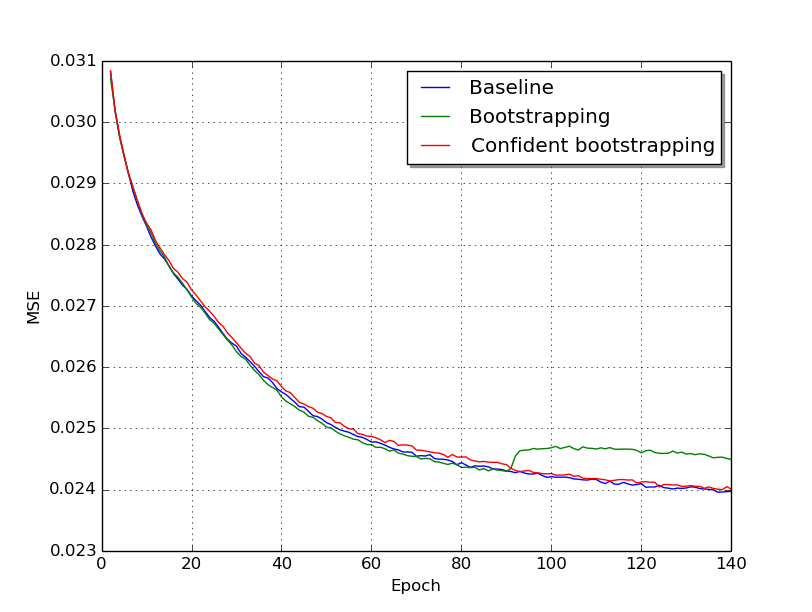
\includegraphics[width=\linewidth]{figs/E4/E4_lc.png}
\caption{MSE test loss} \label{fig:E4_boot_norway_vbase_loss}
\end{subfigure}
\hspace*{\fill} % separation between the subfigures
\begin{subfigure}{0.48\textwidth}
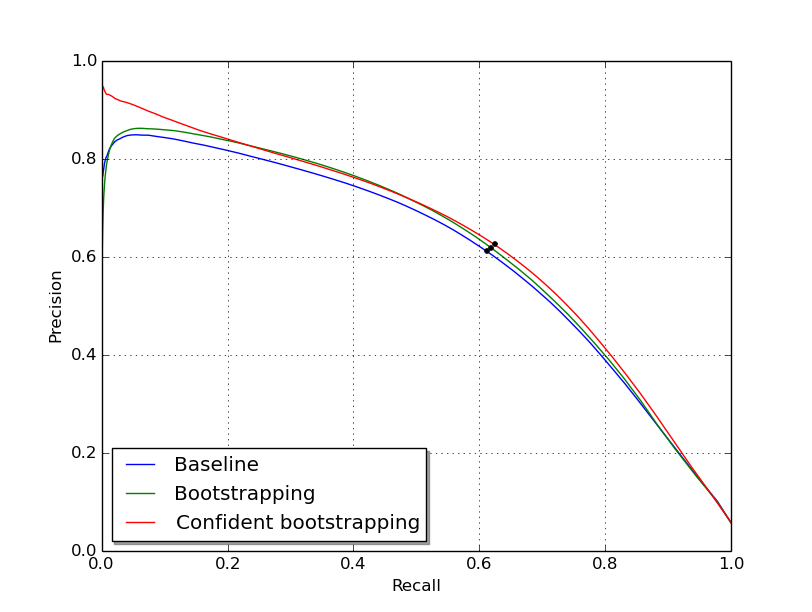
\includegraphics[width=\linewidth]{figs/E4/E4_pr.png}
\caption{Precision and recall comparison.} \label{fig:E4_boot_norway_vbase_pr}
\end{subfigure}
\hspace*{\fill} % separation between the subfigures
\caption{E4 - Comparison of loss functions for Norwegian Roads Dataset Vbase. The training set consists of labels with omission noise, and severe levels registration noise.} \label{fig:E4_boot_norway_vbase}
\end{figure}

\subsection{Road detection system}
\label{sec:results_road_detection_system}
Furthermore, the images in Figure \ref{fig:E6_performance} illustrate qualitatively the performance of the system. For this particular test image, the model is able to identify the majority of the roads present, except for an almost imperceptible dirt road on the right side of the image. There are also some prediction errors, such as roads being disconnected, and prediction artefacts in the forest areas. However, the majority of the forest artefacts have low prediction probabilities, and are removed when applying a threshold operation on the probabilities. The threshold value which result in the best precision and recall trade off, is used in this threshold operation.\\

An interesting observation is that the model also correctly predicts small private roads leading up to houses present in the image. Furthermore, the model detects construction roads in the upper left corner. Since these roads are not present in the label image, the model is penalized for making these predictions by the cross-entropy loss function.\\

\begin{figure}[!ht]
\begin{subfigure}{0.48\textwidth}
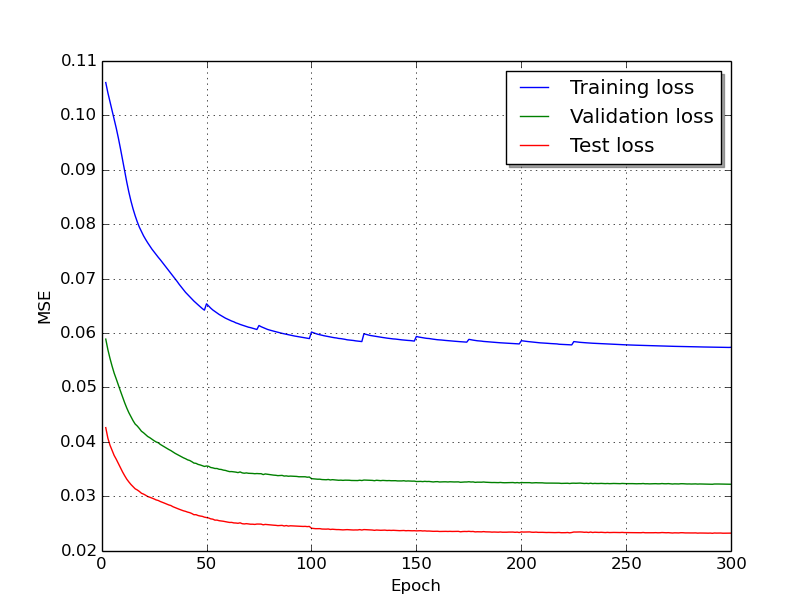
\includegraphics[width=\linewidth]{figs/E6/E6_lc_loss.png}
\caption{MSE loss} \label{fig:E6_performance_mass_lc}
\end{subfigure}
\hspace*{\fill} % separation between the subfigures
\begin{subfigure}{0.48\textwidth}
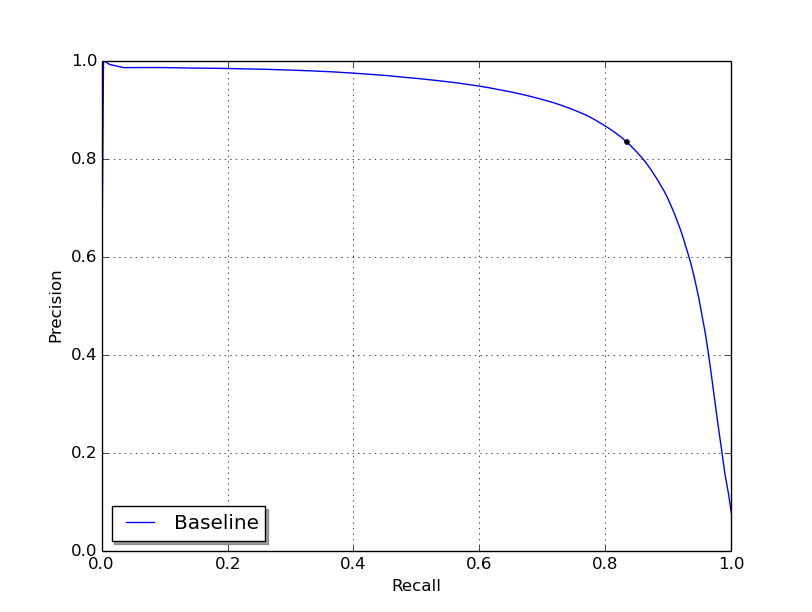
\includegraphics[width=\linewidth]{figs/E6/E6_pr.png}
\caption{Precision and recall.} \label{fig:E6_performance_mass_pr}
\end{subfigure}
\hspace*{\fill} % separation between the subfigures
\caption{E6 - Performance of road detection system trained with Massachusetts Roads Dataset} \label{fig:E6_performance_mass}
\end{figure}

\begin{table}[!ht]
\caption{Curriculum learning results.}
\begin{center}
\begin{adjustbox}{max width=\textwidth}
\begin{tabular}{+l ^r ^r}\hline
\rowstyle{\bfseries}
  System & breakeven & best network\\\hline
  Road detection system & 0.8341 & 0.84131\\
  Curriculum	 trained system & ? &\\
  \cite{MnihThesis} & 0.8873 & \\
  \cite{saito_building_and_roads} & 0.8866& \\\hline
\end{tabular}
\end{adjustbox}
\end{center}
\label{tab:results_curriculum_learning_breakeven}
\end{table}

\begin{figure}
\begin{subfigure}{0.48\textwidth}
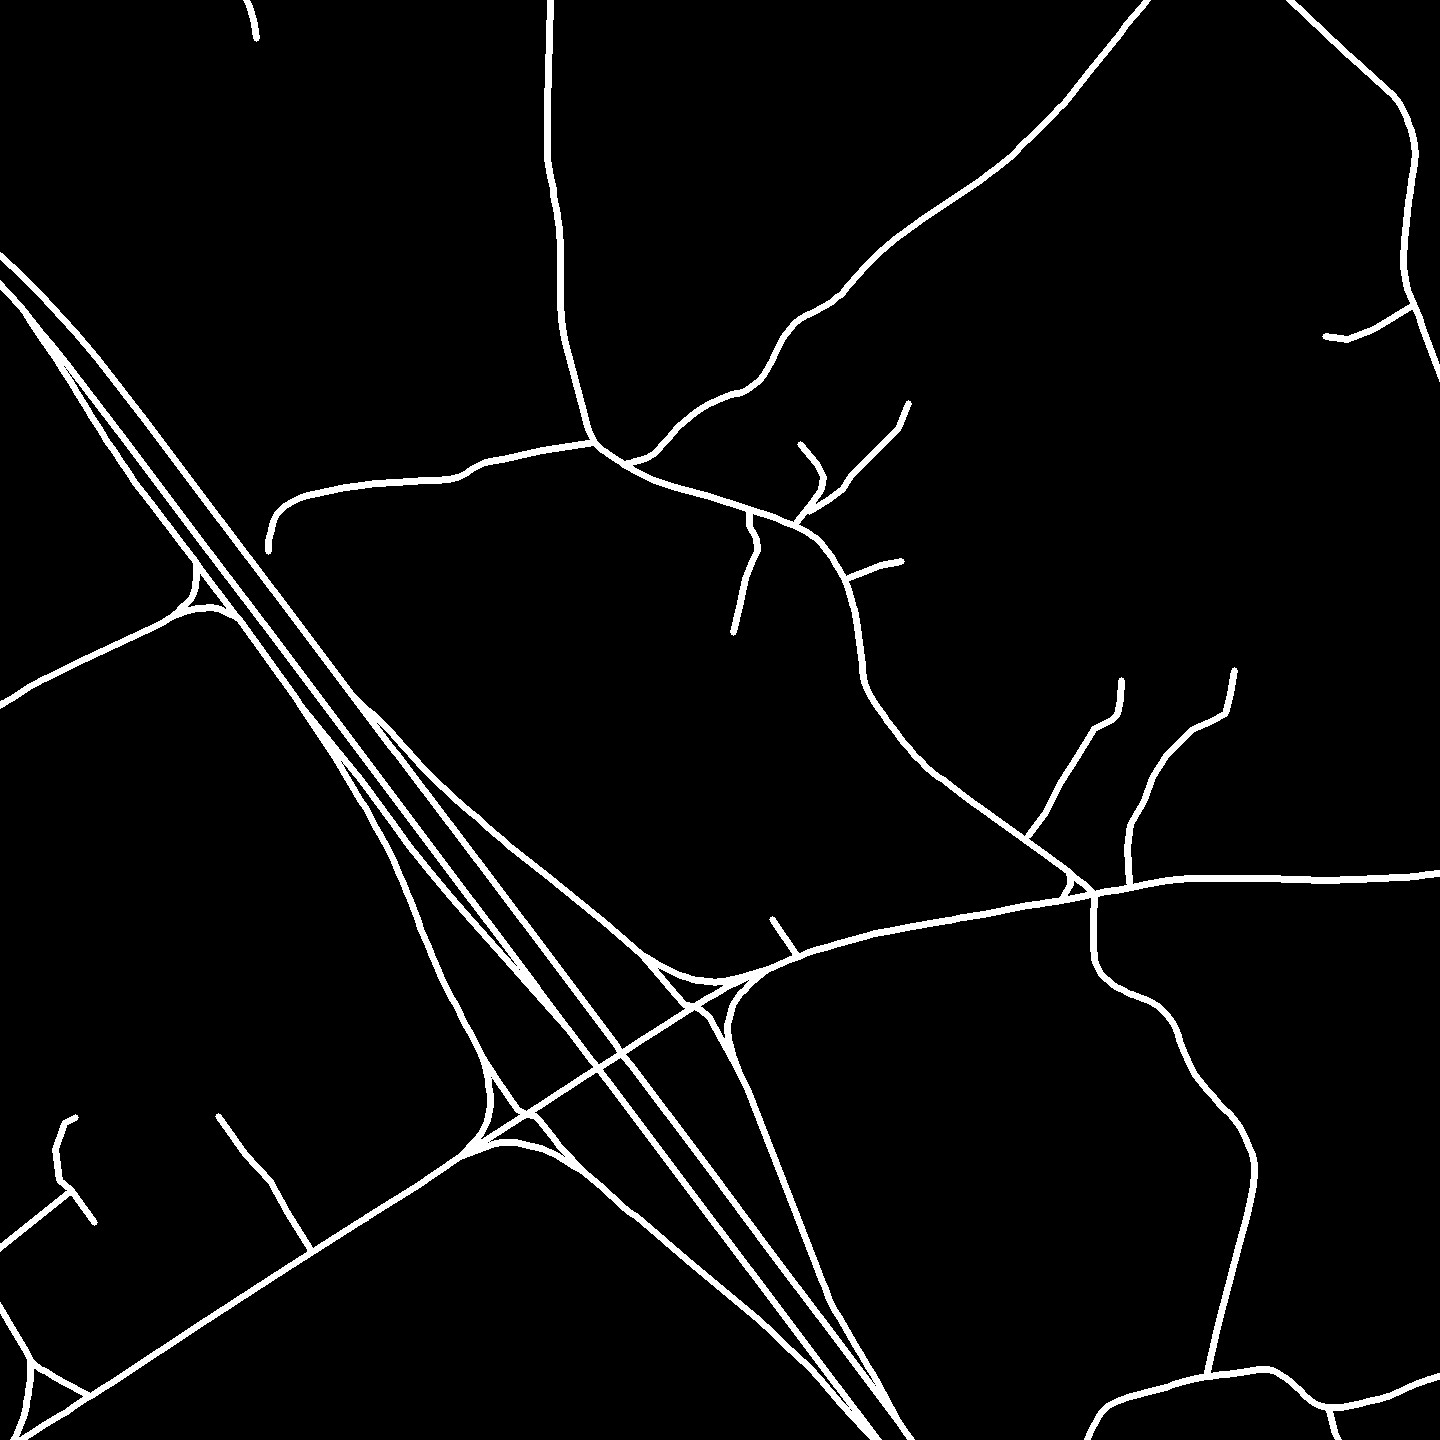
\includegraphics[width=\textwidth]{figs/E6/E6-label.jpg}
\caption{Label image.} \label{fig:E6_label_iamge}
\vspace{0.5cm} % separation vertically between the subfigures
\end{subfigure}
\hspace*{\fill} % separation between the subfigures
\begin{subfigure}{0.48\textwidth}
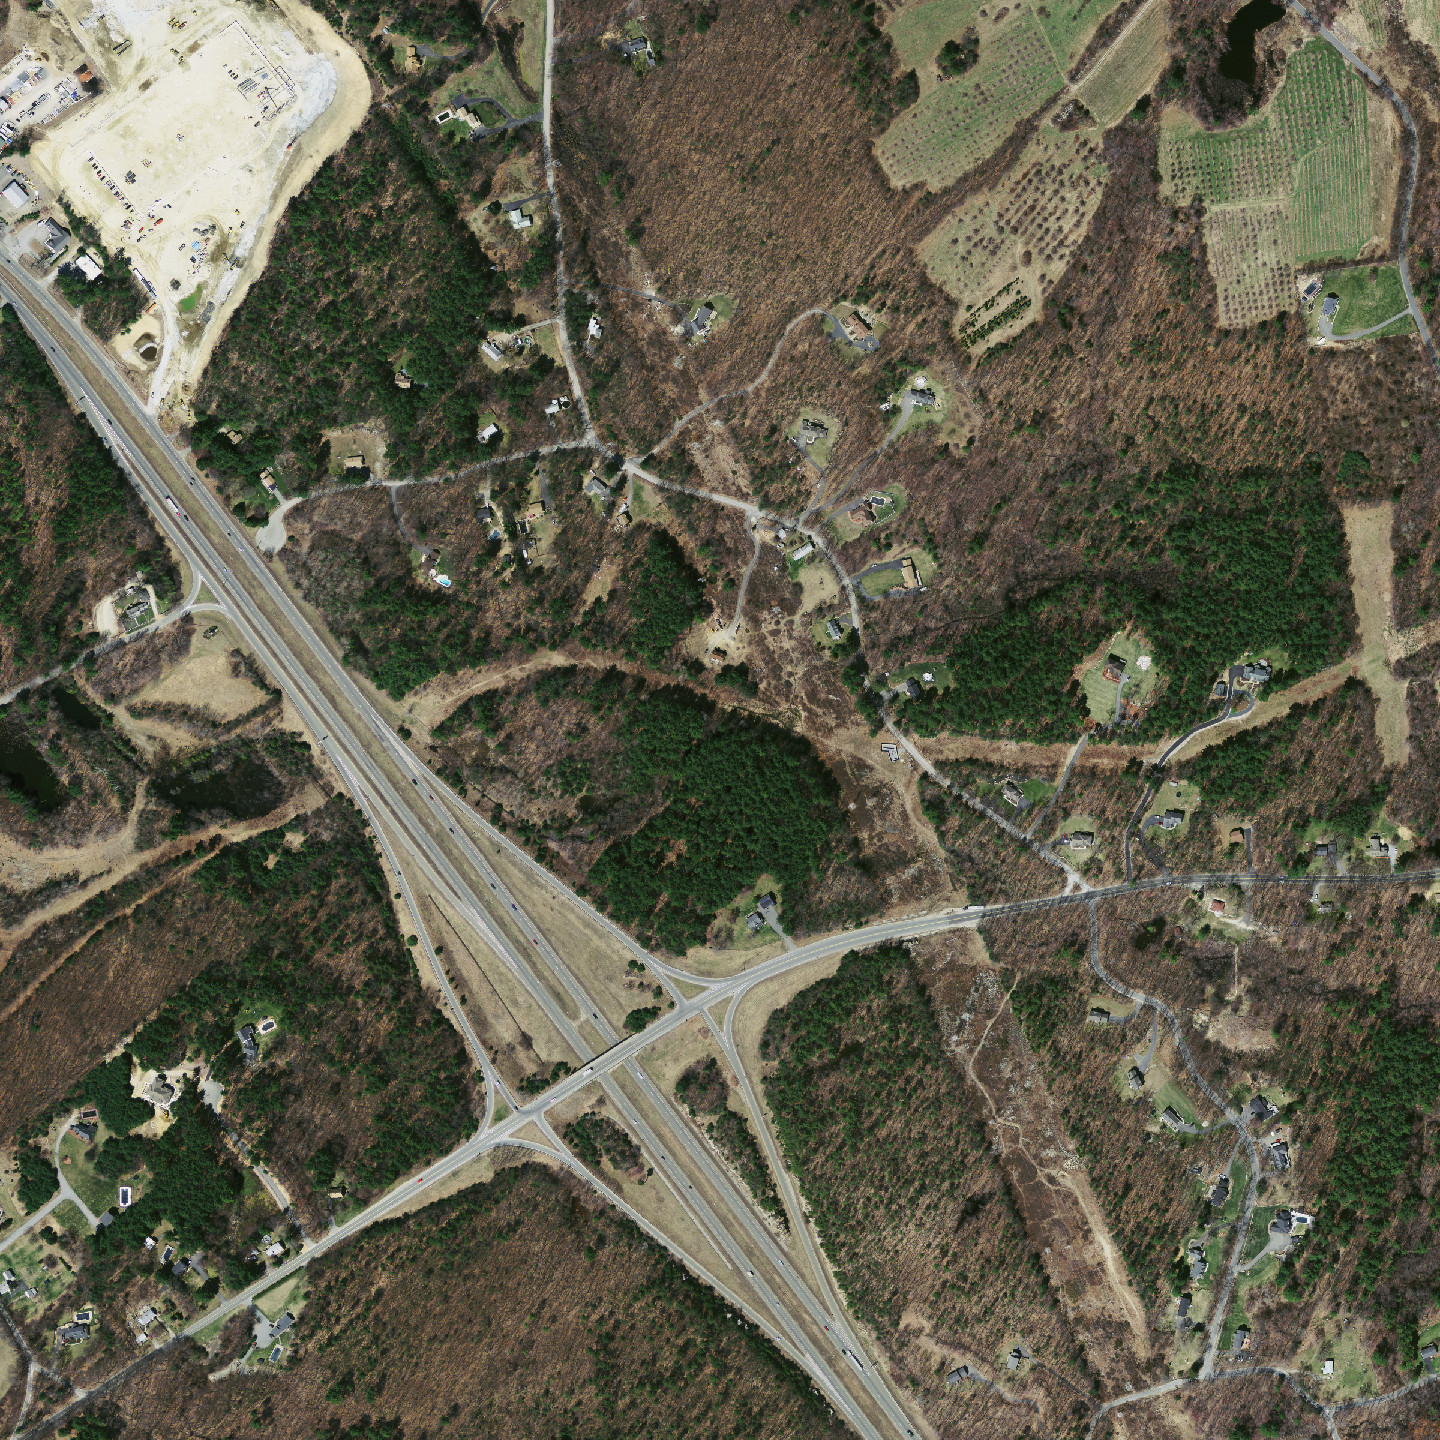
\includegraphics[width=\textwidth]{figs/E6/E6-image.jpg}
\caption{Aerial image.} \label{fig:E6_aerial_image}
\vspace{0.5cm} % separation vertically between the subfigures
\end{subfigure}

\begin{subfigure}{0.48\textwidth}
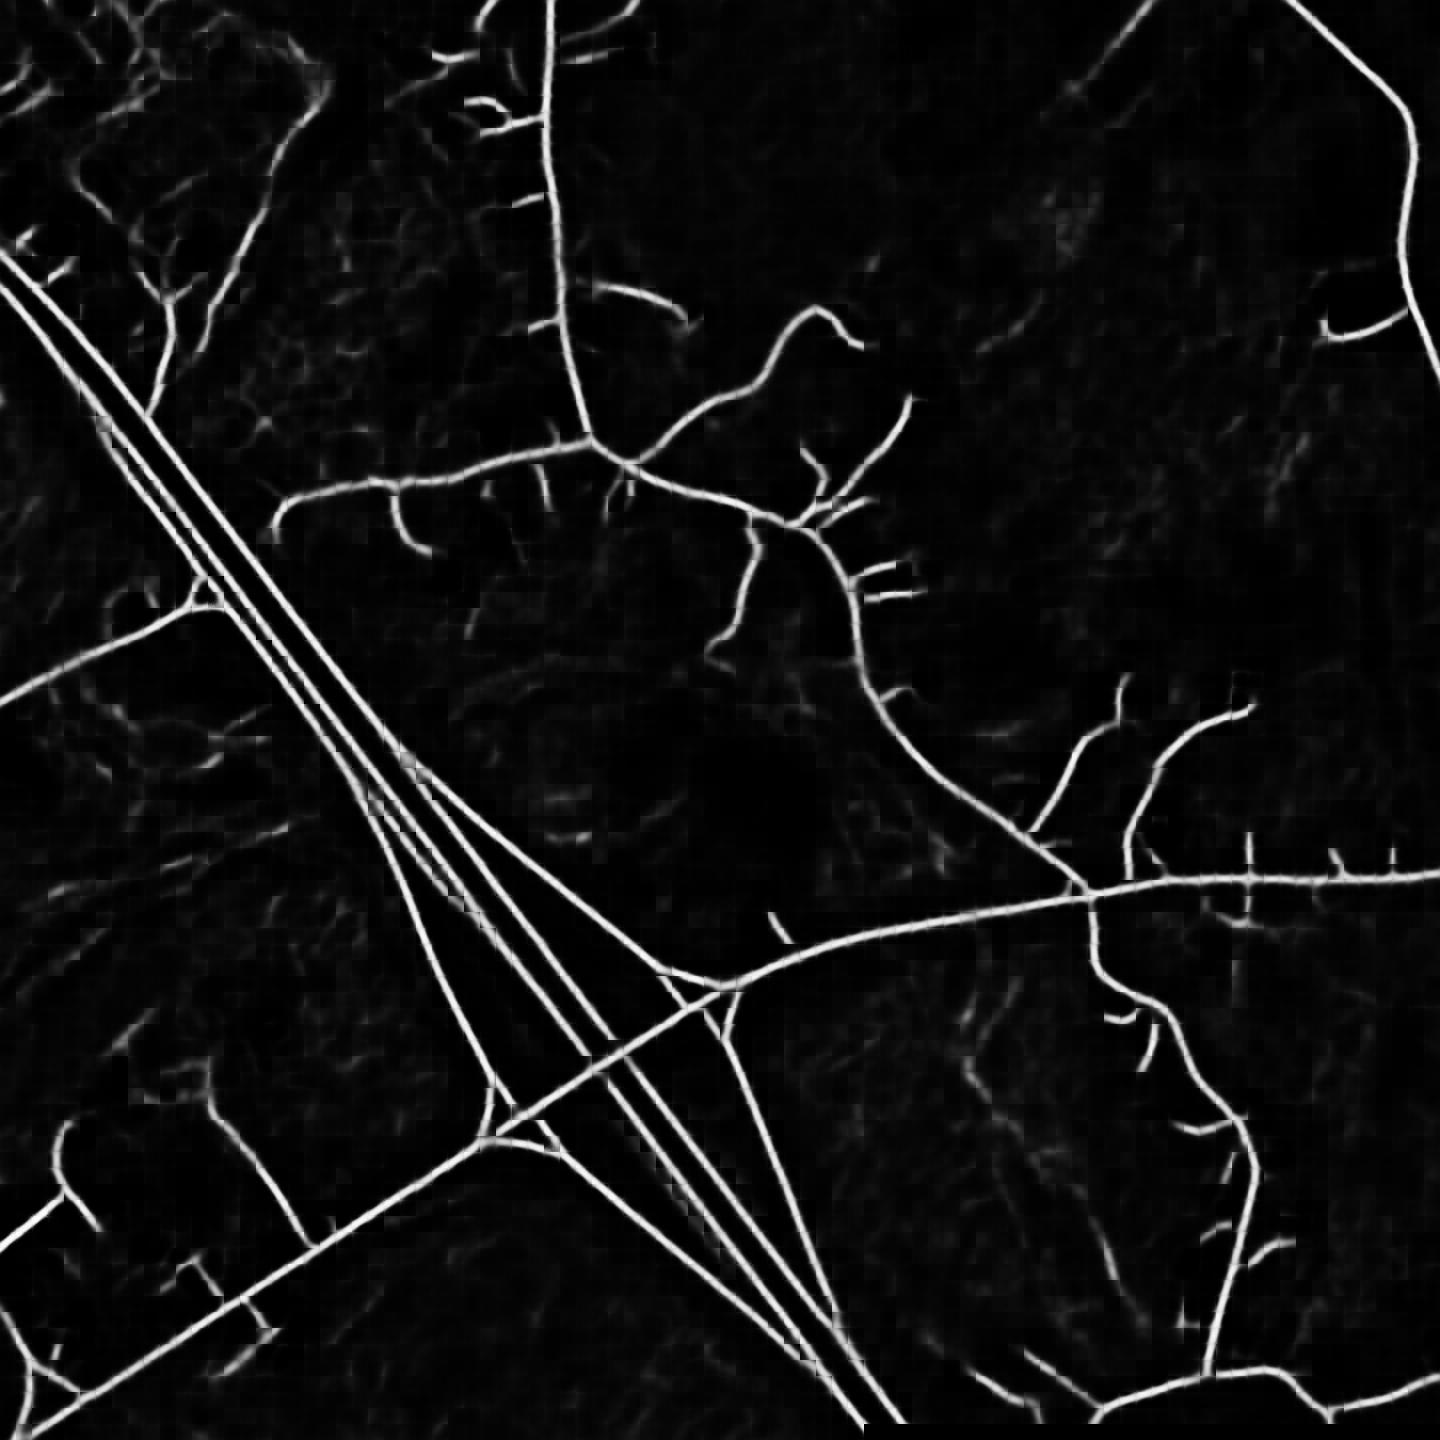
\includegraphics[width=\textwidth]{figs/E6/E6-pred.jpg}
\caption{Model predictions.} \label{fig:E6_model_predictions}
\end{subfigure}
\hspace*{\fill} % separation between the subfigures
\begin{subfigure}{0.48\textwidth}
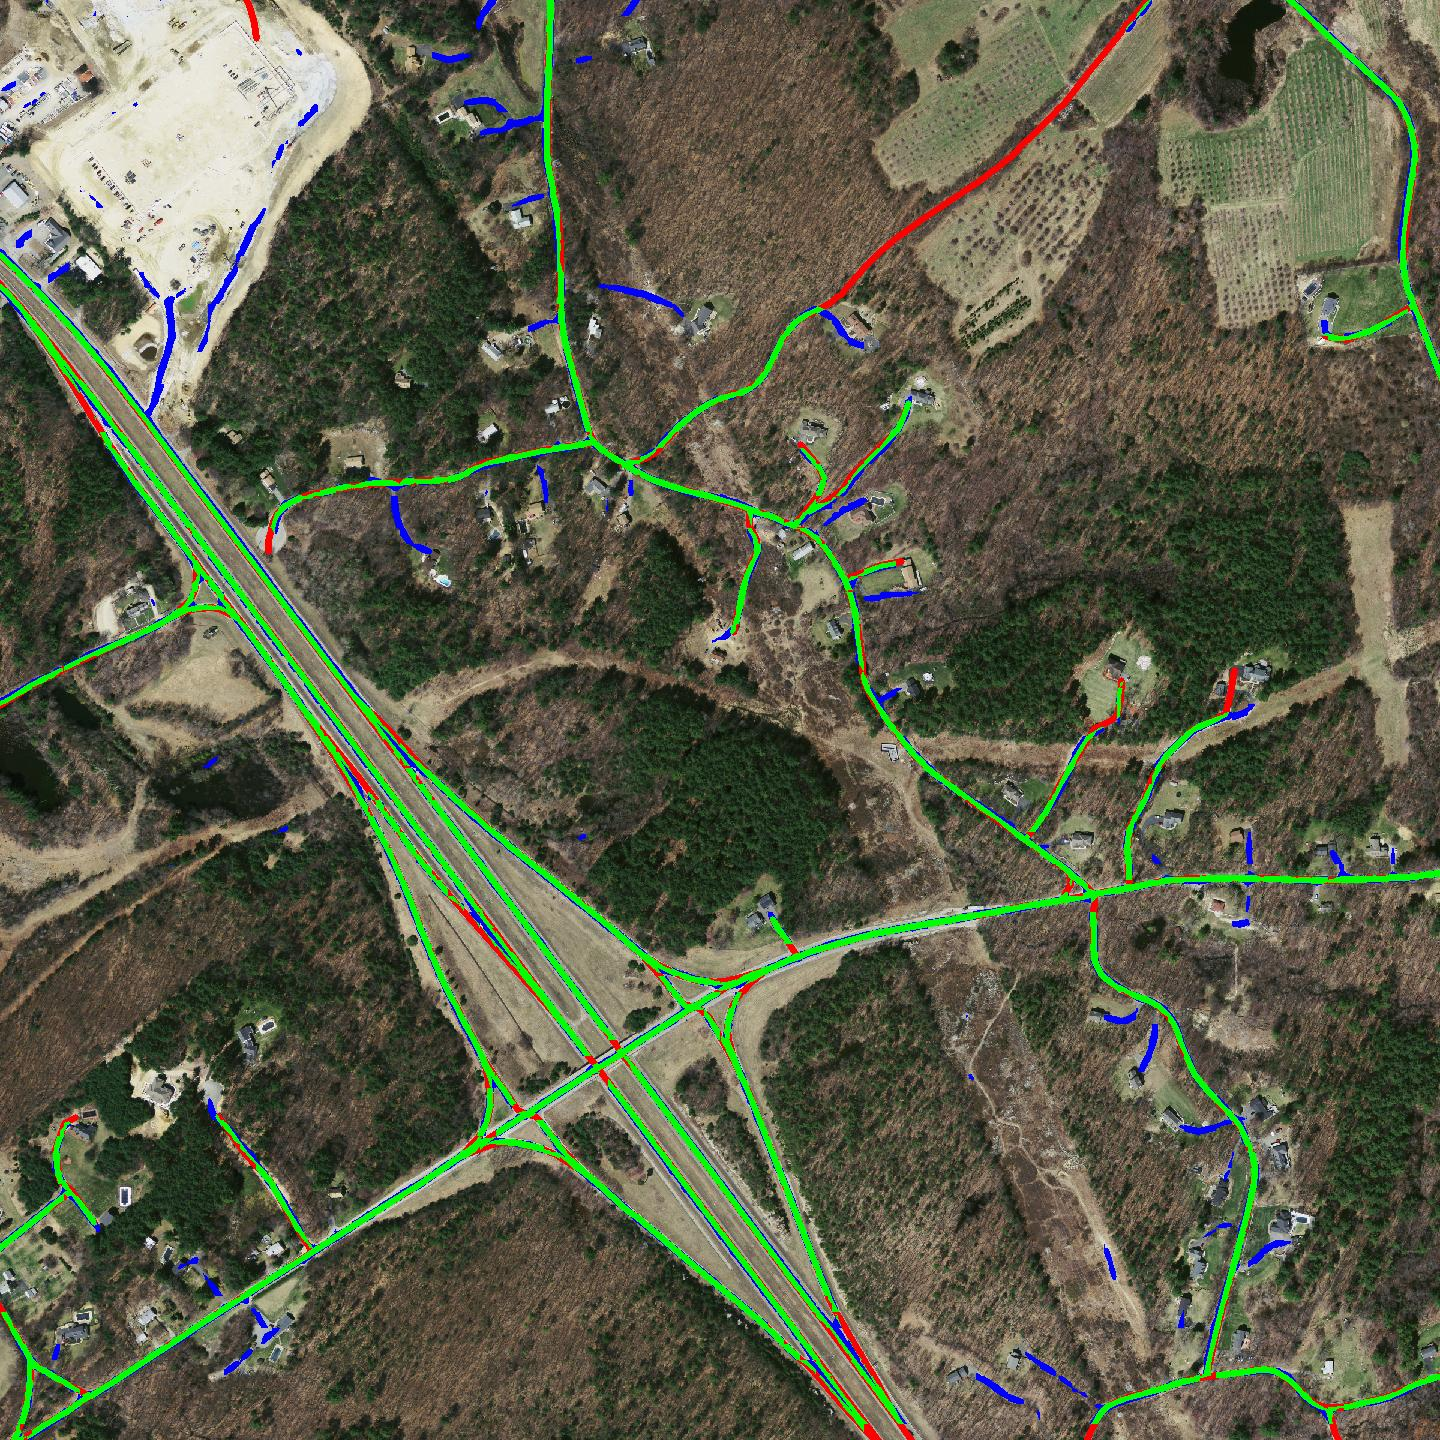
\includegraphics[width=\textwidth]{figs/E6/E6-hit.jpg}
\caption{Prediction hit and miss image.} \label{fig:E6_hit_iamge}
\end{subfigure}
\caption{E6 - Example of model's road detection performance. The aerial image is part of the test set in Massachusetts Roads Dataset} \label{fig:E6_performance}
\end{figure}




\todo[inline]{Choose what to present}
\todo[inline]{Present results for each experiment}
\todo[inline]{Avoid drawing grand conclusions. Only what your data can support}
\todo[inline]{Study tables graphs for unusual things that might raise questions with the reader}
\todo[inline]{Reason for this is the use of 50/50 split. Even though 40 percent is removed the sampling still pick out samples so that 50 percent of patches contain road class pixels. In discussion?}